%%%%%%%%%%%%%%%%%%%%%%%%%%%%%%%%%%%%%%%%%%%%%%
% Head matter - can we try to be consistent on
% included packages
\documentclass{beamer}
\mode<presentation>
{\usetheme{default}
 \usecolortheme{default}
 \usefonttheme{default}
 \setbeamertemplate{navigation symbols}{}
 \setbeamertemplate{footline}[frame number]
% \setbeamertemplate{caption}[numbered]
 }
\usepackage[english]{babel}
\usepackage{algorithm}
\usepackage[noend]{algpseudocode}
\usepackage[utf8x]{inputenc}
\usepackage{graphicx}
\usepackage{hyperref}
%\graphicspath{{./images/}}
\usepackage{tikz}
\usetikzlibrary{shapes.geometric, arrows,chains}
\usepackage{booktabs,makecell,multirow,tabularx}
\usepackage{verbatim}
\renewcommand{\arraystretch}{1.2}
\renewcommand\theadfont{\normalfont\bfseries}
\usepackage{array}
\usepackage{listings}
\lstset{language=Java, showstringspaces=false}
\usepackage[normalem]{ulem}
\usepackage{bm}
\def\layersep{2.5cm}

\usepackage{xcolor}
%\usepackage{subfig}
\setbeamertemplate{caption}{\insertcaption}
\usepackage[caption=false]{subfig}
\usepackage{hyperref}
\usepackage{verbatim}
%\setbeamertemplate{caption}[numbered]%\numberwithin{figure}{section}
% Define block styles
\tikzstyle{decision} = [diamond, draw, fill=blue!20, 
    text width=4.5em, text badly centered, node distance=3cm, inner sep=0pt]
\tikzstyle{block} = [rectangle, draw, fill=blue!20, 
    text width=3em, text centered, rounded corners, minimum height=3em]
\tikzstyle{line} = [draw, -latex']
\tikzstyle{cloud} = [draw, ellipse, fill=red!20, node distance=3cm,
    minimum height=2em]
\tikzset{
  startstop/.style={
    rectangle, 
    rounded corners,
    minimum width=3cm, 
    minimum height=1cm,
    align=center, 
    draw=black, 
    fill=red!30
    },
  process/.style={
    rectangle, 
    minimum width=3cm, 
    minimum height=1cm, 
    align=center, 
    draw=black, 
    fill=blue!30
    },
  decision/.style={
    rectangle, 
    minimum width=3cm, 
    minimum height=1cm, align=center, 
    draw=black, 
    fill=green!30
    },
  arrow/.style={thick,->,>=stealth},
  dec/.style={
    ellipse, 
    align=center, 
    draw=black, 
    fill=green!30
    },
}
\tikzstyle{arrow} = [thick,->,>=stealth]

\tikzset{onslide/.code args={<#1>#2}{%
  \only<#1>{\pgfkeysalso{#2}} % \pgfkeysalso doesn't change the path
}}

\makeatletter
\newenvironment<>{btHighlight}[1][]
{\begin{onlyenv}#2\begingroup\tikzset{bt@Highlight@par/.style={#1}}\begin{lrbox}{\@tempboxa}}
{\end{lrbox}\bt@HL@box[bt@Highlight@par]{\@tempboxa}\endgroup\end{onlyenv}}

\newcommand<>\btHL[1][]{%
  \only#2{\begin{btHighlight}[#1]\bgroup\aftergroup\bt@HL@endenv}%
}
\def\bt@HL@endenv{%
  \end{btHighlight}%   
  \egroup
}
\newcommand{\bt@HL@box}[2][]{%
  \tikz[#1]{%
    \pgfpathrectangle{\pgfpoint{1pt}{0pt}}{\pgfpoint{\wd #2}{\ht #2}}%
    \pgfusepath{use as bounding box}%
    \node[anchor=base west, fill=orange!30,outer sep=0pt,inner xsep=1pt, inner ysep=0pt, rounded corners=3pt, minimum height=\ht\strutbox+1pt,#1]{\raisebox{1pt}{\strut}\strut\usebox{#2}};
  }%
}
\makeatother




%%%%%%%%%%%%%%%%%%%%%%%%%%%%%%%%%%%%%%%%%%%%%%
% Formatting for title page
\title[Deep Learning]{LSTMs and GRUs}
\author{Kate Farrahi}
\institute{ECS Southampton}
\date{\today}
%%%%%%%%%%%%%%%%%%%%%%%%%%%%%%%%%%%%%%%%%%%%%%
\begin{document}
\begin{frame}
  \titlepage
\end{frame}
%-------------------------------------------------------------%

\begin{frame}[fragile]{pause}\frametitle{Vanishing Gradients in RNNs}
The influence of a given input on the hidden layer, and therefore
on the network output, decays as it cycles
around the network's recurrent connections. This effect is referred to as the vanishing gradient problem.
\end{frame}
%-------------------------------------------------------------%

\begin{frame}[fragile]{pause}\frametitle{Vanishing Gradients in RNNs}
\begin{center}
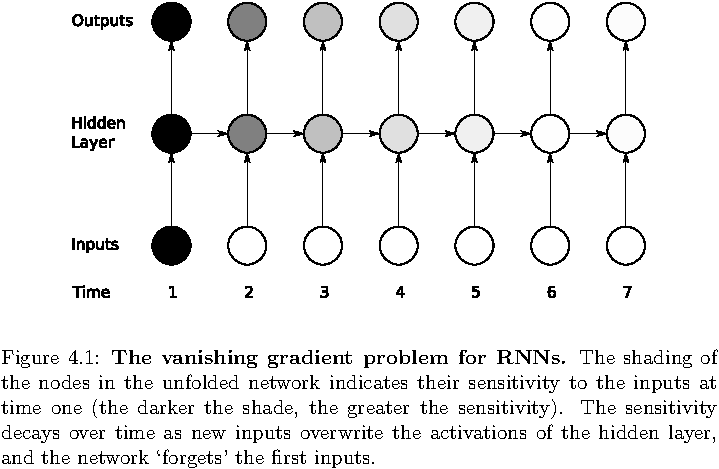
\includegraphics[width=10cm]{vangrad.pdf} \footnote{Graves, Alex. Supervised sequence labelling with recurrent neural networks. Springer, Berlin, Heidelberg, 2012. }
\end{center}
\end{frame}
%-------------------------------------------------------------%

\begin{frame}[fragile]{pause}\frametitle{Vanishing Gradients in RNNs}

\begin{itemize}
\item RNNs have difficulties learning long-range dependencies, i.e. interactions between words that are several steps apart.
\item For example, consider the subject-verb agreement in the sentences below:
\item {\em Our experiments} are based on a variety of datasets to observe the information trajectory of cascade learning and {\em show} consistency across the results.
\item  {\em Our experiment} is based on a variety of datasets to observe the information trajectory of cascade learning and {\em shows} consistency across the results.
\end{itemize}
\end{frame}
%-------------------------------------------------------------%

\begin{frame}[fragile]{pause}\frametitle{Long Short-Term Memory (LSTM)}
\begin{itemize}
\item LSTM was proposed in 1997 by S. Hochreiter and J. Schmidhuber \footnote{Hochreiter, S., and J. Schmidhuber. "Long short-term memory." Neural computation 9.8 (1997): 1735-1780.}
\item The initial version of LSTM block included cells, input and output gates.
\item In 1999, Felix Gers and his advisor J. Schmidhuber and Fred Cummins introduced the forget gate into LSTM architecture, enabling the LSTM to reset its own state.
\item In 2014, K. Cho et al. put forward a simplified variant called Gated recurrent unit (GRU)\footnote{Cho, K.; van Merrienboer, B.; Gulcehre, C.; Bahdanau, D.; Bougares, F.; Schwenk, H.; Bengio, Y. (2014). "Learning Phrase Representations using RNN Encoder-Decoder for Statistical Machine Translation". arXiv:1406.1078}.
\end{itemize}
\end{frame}
%-------------------------------------------------------------%

\begin{frame}[fragile]{pause}\frametitle{LSTM Memory Block}
\begin{center}
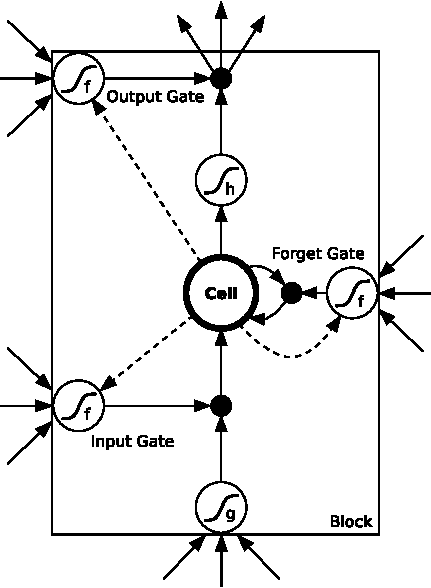
\includegraphics[width=5.5cm]{lstm_fig.pdf} \footnote{Graves, Alex. Supervised sequence labelling with recurrent neural networks. Springer, Berlin, Heidelberg, 2012. }
\end{center}
\end{frame}
%-------------------------------------------------------------%


\begin{frame}[fragile]{pause}\frametitle{LSTM Network}
\begin{center}
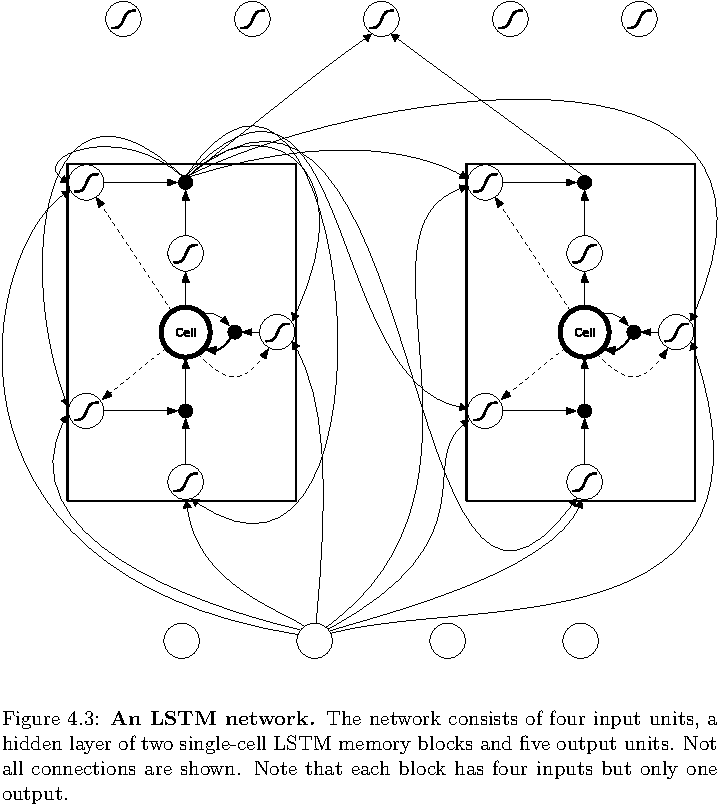
\includegraphics[width=6.5cm]{lstmnet.pdf} \footnote{Graves, Alex. Supervised sequence labelling with recurrent neural networks. Springer, Berlin, Heidelberg, 2012.}
\end{center}
\end{frame}
%-------------------------------------------------------------%

\begin{frame}[fragile]{pause}\frametitle{LSTM Network}
\begin{itemize}
\item The multiplicative gates allow LSTM memory cells to store and access information over longer periods of time, thereby mitigating the vanishing gradient problem.
\item As long as the input gate remains closed, the activation of the cell will not be overwritten and can be available to the network much later in the sequence.
\item This preservation of information is shown in the next figure.
\end{itemize}
\end{frame}
%-------------------------------------------------------------%


\begin{frame}[fragile]{pause}\frametitle{LSTM preservation of gradient information}
\begin{center}
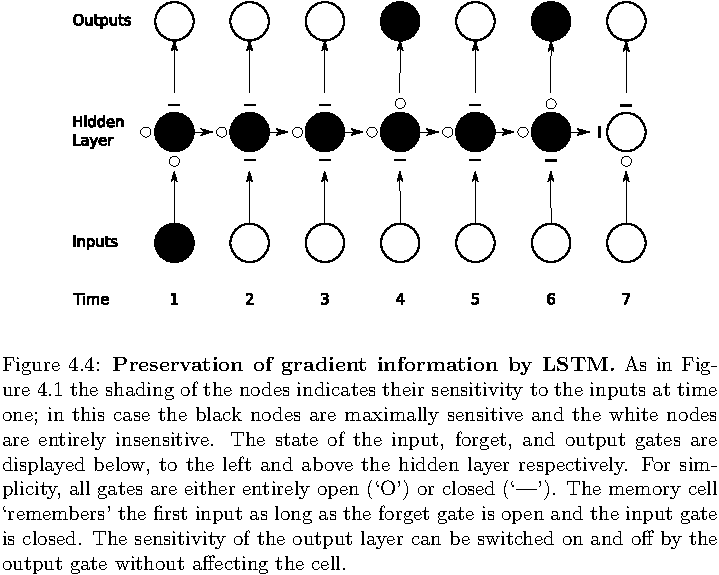
\includegraphics[width=8cm]{lstm_mem.pdf} \footnote{Generating sequences with recurrent neural networks. A Graves - arXiv preprint arXiv:1308.0850, 2013}
\end{center}
\end{frame}
%-------------------------------------------------------------%

\begin{frame}[fragile]{pause}\frametitle{LSTM preservation of gradient information}
Adam's visualisations of LSTMs for COMP6208 are excellent:
\begin{center}
https://secure.ecs.soton.ac.uk/notes/comp6208/lectures/lstm.pdf
\end{center}
\end{frame}
%-------------------------------------------------------------%

\begin{frame}[fragile]{pause}\frametitle{LSTMs}
\begin{eqnarray}
z(t) &=& (x(t), y(t-1)) \\
f(t) &=& \sigma(W_f z(t)) \\
 g(t) &=& \sigma(W_g z(t)) \\
 h(t) &=& tanh(W_h z(t)) \\
 c(t) &=& f(t) \odot c (t-1) + g(t) \odot h(t)\\
 o(t) &=& \sigma(W_o z(t)) \\
y(t) &=& o(t) \odot tanh(c(t)) \\
\end{eqnarray}
\end{frame}
%-------------------------------------------------------------%

\begin{frame}[fragile]{pause}\frametitle{LSTM Success Stories}
\begin{itemize}
\item LSTMs have been used to win many competitions in speech and handwriting recognition
\item Major technology companies including Google, Apple, and Microsoft are using LSTMs as fundamental components in new products. 
\item Google used LSTM for speech recognition on the smartphone, for Google Translate. 
\item Apple uses LSTM for the "Quicktype" function on the iPhone and for Siri. 
\item Amazon uses LSTM for Amazon Alexa.
\item In 2017, Facebook performed some 4.5 billion automatic translations every day using long short-term memory networks \footnote{\url{https://en.wikipedia.org/wiki/Long_short-term_memory}}
\end{itemize}
\end{frame}
%-------------------------------------------------------------%

\begin{frame}[fragile]{pause}\frametitle{Gated Recurrent Unit (GRU)}
\begin{center}
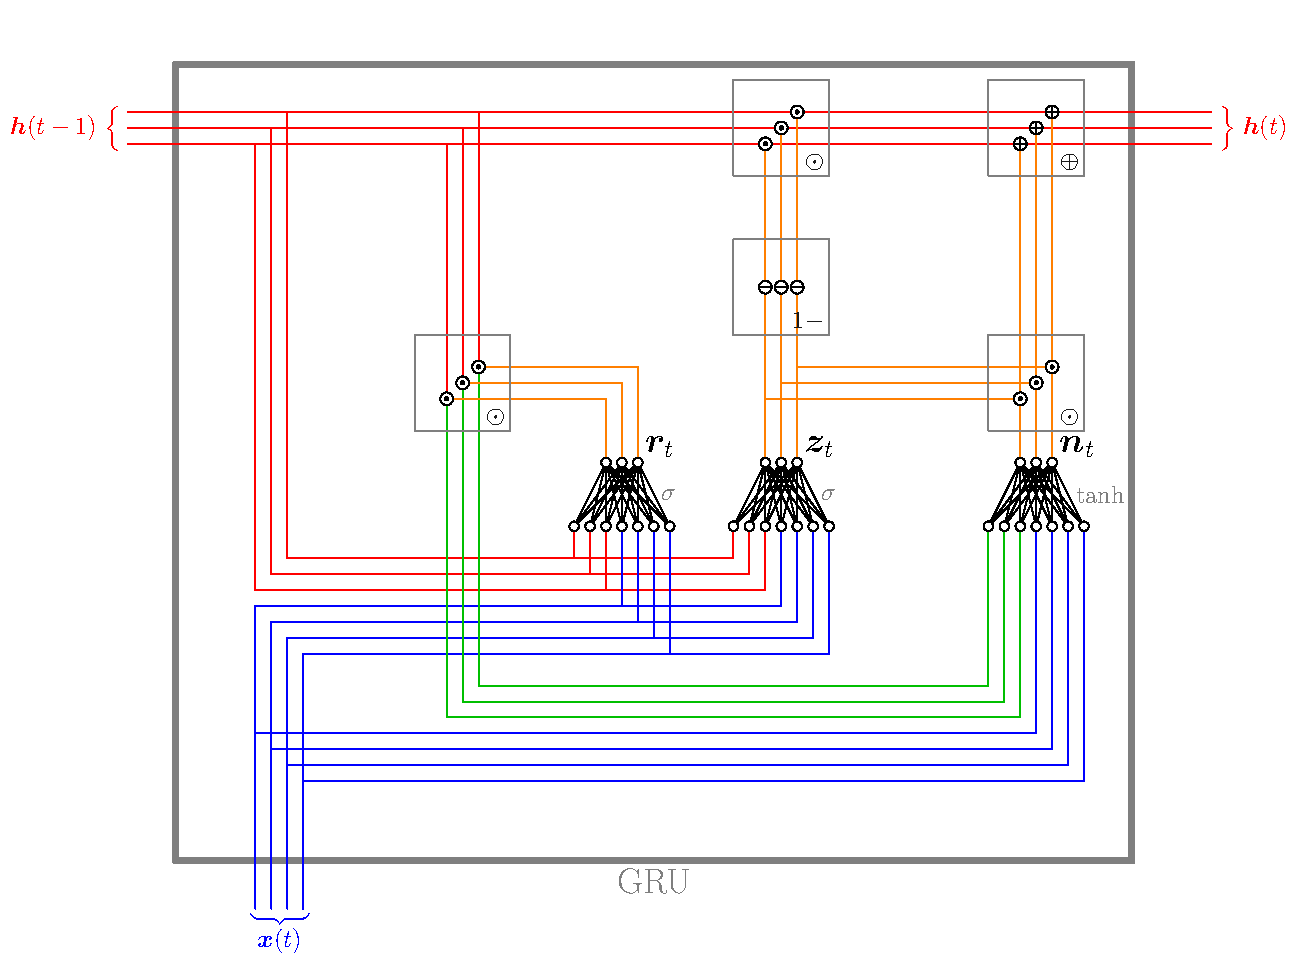
\includegraphics[width=8cm]{GRU.pdf}
\end{center}
\end{frame}
%-------------------------------------------------------------%

\begin{frame}[fragile]{pause}\frametitle{Gated Recurrent Unit (GRU)}
\begin{itemize}
\item $x_t$: input vector
\item $h_t$: output vector
\item $z_t$: update gate vector
\item $r_t$: reset gate vector
\item $W$, $U$, and $b$: parameter matrices and vector
\item $sigm$ or $\sigma_g$ is the sigmoid function
\item $tanh$ or $\sigma_h$ is the hyperbolic tangent
\end{itemize}
\end{frame}
%-------------------------------------------------------------%

\begin{frame}[fragile]{pause}\frametitle{Gated Recurrent Unit (GRU)}
Initially, for $t=0$, $h_0 = 0$
\begin{eqnarray}
z_t &=& \sigma_g (W_z x_t + U_z h_{t-1} + b_z)\nonumber\\\nonumber
r_t &=& \sigma_g (W_r x_t + U_r h_{t-1} + b_r)\\\nonumber
h_t &=& (1 - z_t) \odot h_{t-1} + z_t \odot \sigma_h (W_h x_t + U_h (r_t \odot h_{t-1}) + b_h) \nonumber
\end{eqnarray}
\end{frame}
%-------------------------------------------------------------%

\begin{frame}[fragile]{pause}\frametitle{GRU vs. LSTM?}
\begin{itemize}
\item GRUs have two gates (reset and update) whereas LSTM has three gates (input/output/forget)
\item GRU performance on par with LSTM but computationally more efficient (less complex).
\item In general, if you have a very large dataset then LSTMs will likely perform better. 
\item GRUs are a good choice for smaller datasets.
\end{itemize}
\end{frame}
%-------------------------------------------------------------%

\begin{frame}[fragile]{pause}\frametitle{Regularization in RNNs with LSTM units}
\begin{center}
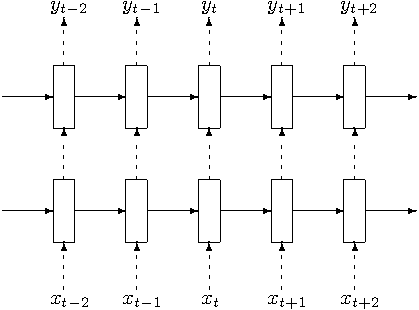
\includegraphics{reg_lstms.pdf}\footnote{\url{https://arxiv.org/pdf/1409.2329.pdf}}
\end{center}
\end{frame}
%-------------------------------------------------------------%

\begin{frame}[fragile]{pause}\frametitle{Regularization in RNNs with LSTM units}
\begin{center}
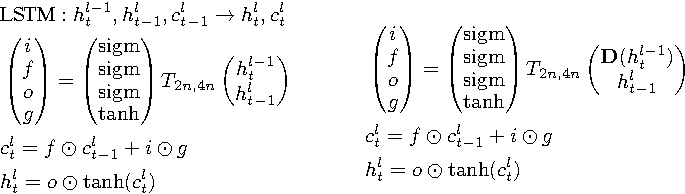
\includegraphics{reglstm_dropout.pdf}\footnote{\url{https://arxiv.org/pdf/1409.2329.pdf}}
\end{center}
\end{frame}
%-------------------------------------------------------------%

\end{document}